




















\section{Our model and training strategy for real-time hit classification}

The goal of our model is to identify \textit{single-hit} while a SPI diffraction
data collection is underway.  From a model perspective, we essentially use the
same neural network architecture to create an experiment-specific hit classifier
and a generalized hit classifier.  We focus more on explaining how our
experiment-specific classifier works, considering it will have an immediate
impact on real-time classification.  We illustrate the training strategy of a
generalized model afterwards.  


\subsection{CNN vision backbone}

Our CNN vision backbone consists of two convolutional layers that extract image
features and two fully connected layers that compress image features into low
dimensional embeddings.  The first convolutional layer uses a $5 \times 5$
single channel filter with a stride of one and no padding.  The second
convolutional layer employs a 32-channel $5 \times 5$ filter with a with a
stride of one and no padding.  A ReLU activation function is applied to the
outcome of each convolutional layer, which is followed by a max-pooling
operation performed by a $2\times 2$ filter with a stride of two.  Then, two
fully connected layer are used to generate the final embedding with the size of
128.  As a result, all SPI diffraction images are encoded into embeddings in a
latent space, where embedding distance between two images, estimated with $L^2$
squared distance, is a measurement of their similarities.  Expectedly,
identically labelled hits should have a small embedding distance, whereas
differently labelled hits should have a large embedding distance.  

% Maybe discuss how many parameters are involved depending on the image cropping
% and downsizing in data preprocess.  

%% row x col x filters
%% \renewcommand{\arraystretch}{1.4}
%% pnCCD: 
\begin{table}
\caption{Our neural network architecture of the image encoder.
{\color{red} This whole table can be replaced by an illustrative figure.}}
%% \resizebox{1.0\textwidth}{!}{
    \begin{tabularx}{\textwidth}{   l | l l l X X  }
        Layer       &  In channels    & Out channels    & Kernel size & Stride       & Padding     \\
        \hline
        Conv 1      &  1              & 32              & 5           & 1            & 0           \\
        ReLU 1      &  \textemdash    & \textemdash     & \textemdash & \textemdash  & \textemdash \\
        MaxPool2D 1 &  \textemdash    & \textemdash     & 2           & 2            & 0           \\
        Dropout 1   &  \textemdash    & \textemdash     & \textemdash & \textemdash  & \textemdash \\
        \hline
        Conv 2      &  32             & 64              & 5           & 1            & 0           \\
        ReLU 2      &  \textemdash    & \textemdash     & \textemdash & \textemdash  & \textemdash \\
        MaxPool2D 2 &  \textemdash    & \textemdash     & 2           & 2            & 0           \\
        Dropout 2   &  \textemdash    & \textemdash     & \textemdash & \textemdash  & \textemdash \\
        \hline
        Layer       &  In features    & Out features    & \textemdash & \textemdash  & \textemdash \\
        \hline
        FC 3        &  *              & 512             & \textemdash & \textemdash  & \textemdash \\
        ReLU 3      &  \textemdash    & \textemdash     & \textemdash & \textemdash  & \textemdash \\
        \hline
        FC 4        &  512            & 128             & \textemdash & \textemdash  & \textemdash \\
    \end{tabularx}
%% }
\end{table}


\subsection{Triplet loss function for training}

How to train the CNN vision backbone to distinguish SPI hits?  We use a strategy
adopted from FaceNet \cite{schroffFaceNetUnifiedEmbedding2015} that uses a
triplet loss function for training the vision backbone.  Each input consists of
a triplet of diffraction images, which are called an anchor $x^a$, a positive
$x^p$ and a negative $x^n$. The anchor shares the same label as the positive but
different from the negative.  Two pairs will be put into a comparison in the
model. The postive pair contains the anchor and the positive $(x^a, x^p)$,
whereas the negative pair include the anchor and the negative $(x^a, x^n)$.
During training, three identical CNNs $f$ extract features from a triplet $(x^a,
x^p, x^n)$, while another component in the model measures the squared $L_2$
distance in the positive pair $\|f(x^a) - f(x^p)\|_2^2$ and the negative pair
$\|f(x^a) - f(x^n) \|_2^2$, respectively.  The objective of training our CNN $f$
is to separate the negative pair $(f(x^a), f(x^n))$ more than the the positive
pair $(f(x^a), f(x^p))$ by at least a margin $\alpha$.  Suppose there are $N$
triplets, the objective can be stated as 

\newcommand{\isep}{\mathrel{{.}\,{.}}\nobreak}
\begin{equation} \label{eq:objective}
    \begin{array}{l}
       \|f(x_i^a) - f(x_i^p)\|_2^2 + \alpha < \|f(x_i^a) - f(x_i^n)\|_2^2, \, i = 1 \isep N
    \end{array}
\end{equation}

Meanwhile, we enforce that every embedding has a unit length of one in a
$d$-dimensional latent space, namely $f(x) \in \mathbb{R}^d$ and $\|f(x)
\|_2=1$. It means that a SPI diffraction image will be mapped to a single point
on a $d$-dimensional hypersphere with a radius of one.  We can expect
identically labelled hits will get closer over the course of training and
eventually form a cluster.  The average distance between two clusters will
ultimately be at least $\alpha$ in a squared $L_2$ norm sense. The largest value
of a possible $\alpha$ is 4. Since we consider only three classes, there is
plenty of room to fit them on a hypersphere.  As a result, the value of $\alpha$
can take on many values.  FaceNet choose a very small $\alpha$ because they need
to fit millions of classes onto a hypersphere and clusters have to sit close to
one another.  

To facilite the training, the objective in Eq. (\ref{eq:objective}) is turned into the
triplet loss function in Eq. (\ref{eq:triplet_loss}).

\begin{equation} \label{eq:triplet_loss}
    \sum_{i=1}^{N} \left[ \alpha + \|f(x_i^a) - f(x_i^p)\|_2^2 - \|f(x_i^a) -
    f(x_i^n)\|_2^2 \right]_+
\end{equation}


\subsection{Selection of semi-hard triplets}

A triplet can be drawn completely randomly in three steps: (1) Randomly choose
one class;  (2) Randomly sample two examples from the chosen class;  (3)
Randomly sample one example from any class other than the chosen class.  This
method, despite being easy to implement, might not deliver fast convergence when
there are many easy triplets.  We consider three kinds of triplets that might
exist during model training: easy, semi-hard and hard shown in Fig. (\ref{fig:
semi-hard}).  In an easy triplet, the negative example is already separated by
at at leats a margin of $\alpha$ than the positive example.  In a hard triplet,
the negative example is actually closer to the anchor than the positive is.  In
a semi-hard triplet, the negative example still stays more apart from the anchor
than the positive example does, but the margin is smaller than $\alpha$.  The
problem with easy triplets is that they contribute to zero in the triplet loss,
and thus the training adjusts the model weights according to other triplets. The
problem with too many hard examples is that hard examples are more likely to be
a small fraction of samples, and minimization routine will prioritize the
separation of those few hard examples from the anchor that can lead to bad local
minima.  Therefore, it's a more reasonable option to select semi-hard triplets
for training.  This strategy doesn't mean to ignore hard examples at all.
Instead, once hard examples are pulled into the semi-hard zone, minimization can
eventually pull them into the easy zone. This way allows majority of the
negative examples to stay away from the anchor by a considerable margin
$\alpha$.  From a practical standpoint, the selection of semi-hard triplets is
done at the mini-batch level, where our model randomly selects a triplet that
satisfies the following condition.  

\begin{equation}\label{eq: semi-hard condition}
    \begin{aligned}[b]
    &\|f(x_i^a) - f(x_i^p)\|_2^2 \;<\; \|f(x_i^a) - f(x_i^n)\|_2^2 \;<\;
    \|f(x_i^a) - f(x_i^p)\|_2^2 + \alpha, \\
    &i = 1 \isep N
    \end{aligned}
\end{equation}

\begin{figure} 
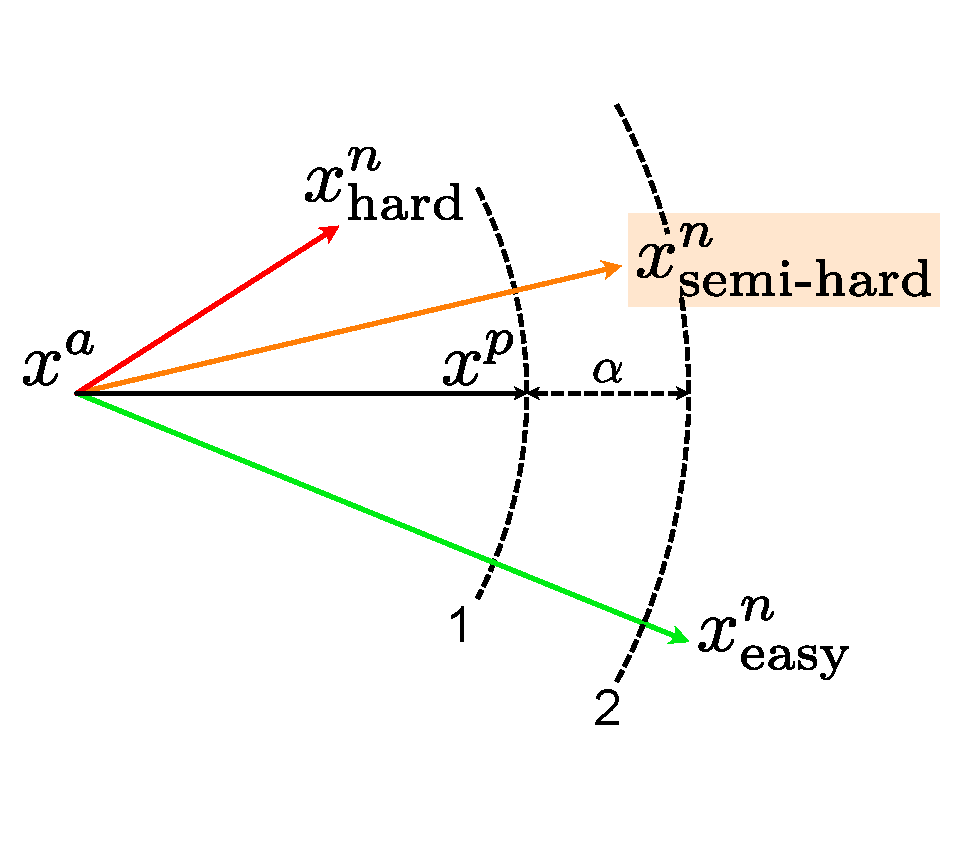
\includegraphics[width=1.0\textwidth,keepaspectratio]
{./figures/triplet_difficulty_level.pdf} 

\caption{An example semi-hard triplet in 2D.  For illustration purposes, the
hypersphere constraint is not enforced.  A positive example $x^p$ sits exactly
on the boundary 1, which is an arc centered at $x^a$. Boundary 2 is $\alpha$
apart from $x^p$ and concentric to boundary 1.  Hard examples are located inside
boundary 1.  Easy examples are located beyound boundary 2. Semi-hard examples
are located in between boundary 1 and 2.  } 

\label{fig: semi-hard} 
\end{figure}


\subsection{Optimization}

%% Adam optimization algorithm

We trained our neural network models using Adam
\cite{kingmaAdamMethodStochastic2017} with the learning rate of $10^{-3}$.  The
model weights are initialized to random values from a Gaussian probability
distribution with a mean of $0.0$ and a standard deviation of $0.2$.  

\subsection{Data preprocessing}

The reasons of employing data preprocessing are three-fold in our application:
highlight features, upscale datasets and reduce image size.  Firstly, a typical
way to highlight image features is to zoom in on the region of interest (ROI) if
available.  In SPI diffraction images, features are predominantly located near
the X-ray beam center and areas remote to the center have much weaker signals.
Based on this observation, we decide to do image cropping by only keeping the
pixels in a user-specified ROI.  Secondly, a diffraction image collected in a
SPI experiment won't change its nature after an in-plane rotation with the beam
path as the rotational axis.  This characteristic allows us to upscale our
dataset by applying random in-plane rotation, which ultimately teaches our model
that a particular form of diffraction image can re-appear in an experiment
except it differs by some rotation.  It's worth noting that any hit class, e.g.
\textit{single-hit}, can have various forms but random rotation cannot alter any
unique form of a class to resemble another one.  Lastly, we downsample
diffraction images in our dataset by a factor of 6.  We don't have an evidence
to conclude that the factor of 6 gives the best trade-off between size reduction
and feature quality.  Instead, we found this value in practice that it gives
good performance in our application.  
